\section{A loss budget for nested idempotents}
\label{nest:section}

For idempotents in a semigroup, write $d\trianglelefteq e$ if
$de=ed=d$, and say that $d$ is \emph{nested under} $e$.
This is a partial order: reflexivity and antisymmetry are immediate,
and if $d\trianglelefteq e\trianglelefteq f$, then
$df=(de)f=d(ef)=de=d$ and $fd=f(ed)=(fe)d=ed=d$.
Nesting is distinct from the edge-inclusion order $\sqsubseteq$.

We will bound the sum of the losses incurred along a nested chain,
even though the identity, the recurrent classes, and hence the meaning
of a loss change at every step. The key fact is a containment dichotomy:
a new recurrent class contains either an old class that is not lost,
or at least two old classes.

\begin{lemma}[Absorption under nesting]
\label{nest:absorption}
Let $d,e\in\mathcal T_m$ be idempotents with $d\trianglelefteq e$.
For either sign $\sigma$,
\[
 K_e^\sigma\subseteq K_d^\sigma,
 \qquad
 P_e^\sigma P_d^\sigma\subseteq P_d^\sigma,
 \qquad
 P_d^\sigma P_e^\sigma\subseteq P_d^\sigma.
\]
In the positive sign one also has
\begin{equation}
\label{nest:through-absorption}
 F_eP_d^+\subseteq P_d^+,
 \qquad P_d^+F_e\subseteq P_d^+.
\end{equation}
The corresponding negative-sign inclusions use $B_e$.
\end{lemma}

\begin{proof}
We prove the positive-sign statements and suppress the superscript $+$.
Because $d\in e\mathcal T_m e$, its returns contain those of $e$:
$L_e\subseteq L_d$ and $R_e\subseteq R_d$.
Set
\[
 S=(L_dR_e)^*,\qquad T=(L_eR_d)^*.
\]
Then $K_e\subseteq S,T\subseteq K_d$.
The multiplication formulas applied to $ed=de=d$ give
\begin{align}
 F_d&=F_eSF_d=F_dTF_e,\label{nest:forward-identities}\\
 L_d&=L_e\cup F_eSL_dB_e,
 &R_d&=R_e\cup B_eR_dTF_e.
 \label{nest:return-identities}
\end{align}

We spell out the two star rearrangements needed below, using the
finite-path identities in \eqref{diag:star}.
Expanding $R_d$ in $K_d=(L_dR_d)^*$, we obtain
\begin{align*}
 K_d
 &=\bigl(L_dR_e\cup L_dB_eR_dTF_e\bigr)^*\\
 &=S\bigl(L_dB_eR_dTF_eS\bigr)^*,\\
 F_eK_dF_d
 &=\bigl(F_eSL_dB_eR_dT\bigr)^*F_eSF_d\\
 &=\bigl(F_eSL_dB_eR_dT\bigr)^*F_d
 \subseteq K_dF_d.
\end{align*}
Indeed, $F_eSL_dB_e\subseteq L_d$ by
\eqref{nest:return-identities}, so the relation inside the last star
is contained in $L_dR_dT\subseteq K_d$.
For the other side, expand $L_d$ instead:
\begin{align*}
 K_d
 &=\bigl(L_eR_d\cup F_eSL_dB_eR_d\bigr)^*\\
 &=T\bigl(F_eSL_dB_eR_dT\bigr)^*,\\
 F_dK_dF_e
 &=F_dTF_e\bigl(SL_dB_eR_dTF_e\bigr)^*\\
 &=F_d\bigl(SL_dB_eR_dTF_e\bigr)^*
 \subseteq F_dK_d.
\end{align*}
Here $B_eR_dTF_e\subseteq R_d$, so the relation inside the star
is contained in $SL_dR_d\subseteq K_d$.
These inclusions, multiplied by the remaining $K_d$, prove
\eqref{nest:through-absorption} because $P_d=K_dF_dK_d$.
Finally, $K_dP_d=P_dK_d=P_d$ and $K_e\subseteq K_d$ imply
\[
 P_eP_d=K_eF_eK_eP_d\subseteq P_d,
 \qquad P_dP_e=P_dK_eF_eK_e\subseteq P_d.
\]
Reflection proves all negative-sign statements.
\end{proof}

\begin{lemma}[Containment of recurrent classes]
\label{nest:containment}
Let $d,e\in\mathcal T_m$ be idempotents with $d\trianglelefteq e$.
Every class in $\mathcal C_d$ contains either
\begin{enumerate}
 \item a whole class in $\mathcal C_e\setminus\mathcal M_e(d)$; or
 \item two distinct whole classes in $\mathcal C_e$.
\end{enumerate}
All classes in either containment have the same sign.
\end{lemma}

\begin{proof}
Again work in the positive sign and omit its superscript.
Fix a recurrent point $x$ of $P_d$.
Using \eqref{nest:forward-identities} twice, its recurrence gives
\[
 x\bigl(K_dF_eSF_dTF_eK_d\bigr)x.
\]
By the rectangle cover in Lemma~\ref{diag:rectangles}, each of the
two displayed $F_e$-edges can be factored through an $e$-recurrent
point. Denote the first point by $p$ and the second by $q$.
The resulting witness has the form
\begin{equation}
\label{nest:factored-witness}
 x\,\alpha\,p\,\beta\,q\,\gamma\,x,
\end{equation}
where
\begin{align*}
 \alpha&=K_dF_eK_e,\\
 \beta&=K_eF_eSF_dTF_eK_e=K_eF_dK_e=U_e^+(d),\\
 \gamma&=K_eF_eK_d.
\end{align*}
Here $\beta\subseteq P_d$ because $K_e\subseteq K_d$.
Moreover, Lemma~\ref{nest:absorption} shows that multiplying $P_d$
on either side by $\alpha$ or $\gamma$ gives a subrelation of $P_d$.
Thus all four endpoint relations needed for class membership follow
from \eqref{nest:factored-witness} and $xP_dx$:
\[
\begin{array}{ll}
 x\,P_d\,x\,\alpha\,p &\Longrightarrow xP_dp,\\
 p\,\beta\,q\,\gamma\,x &\Longrightarrow pP_dx,\\
 x\,\alpha\,p\,\beta\,q &\Longrightarrow xP_dq,\\
 q\,\gamma\,x\,P_d\,x &\Longrightarrow qP_dx.
\end{array}
\]
In particular $p$ and $q$ are recurrent for $P_d$ and belong to the
class of $x$. In the first and last lines, inserting the recurrence
at $x$ is essential: the shorter witness portion alone need not
contain a $d$-through edge.

The entire $P_e$-class of $p$ lies in the $P_d$-class of $x$.
Indeed, if $r$ is in the former class, then
$xP_dpP_er$ and $rP_epP_dx$, and the two mixed absorptions of
Lemma~\ref{nest:absorption} give $xP_dr$ and $rP_dx$.
The same argument applies to $q$.
If their $P_e$-classes are distinct, this proves the second alternative.
If they coincide, then $pU_e^+(d)q$ by
\eqref{nest:factored-witness} and $qP_ep$.
The corner absorption $U_e^+(d)P_e\subseteq U_e^+(d)$ gives
$pU_e^+(d)p$, so that class is not in $\mathcal M_e(d)$.
This proves the first alternative. Reflection handles the negative sign.
\end{proof}

\begin{proposition}[Chain bound]
\label{nest:chain}
Let $b_0,b_1,\ldots,b_k\in\mathcal T_m$ be idempotents such that
$b_j\trianglelefteq b_{j-1}$ for $1\leq j\leq k$.
Suppose a single set $J_0\subseteq\mathcal C_{b_0}$ satisfies
\[
 \mathcal M_{b_0}(b_j)\subseteq J_0
 \qquad(0\leq j\leq k).
\]
Then
\begin{equation}
\label{nest:chain-bound}
 \sum_{j=1}^k\bigl|\mathcal M_{b_{j-1}}(b_j)\bigr|
 \leq 2|J_0|.
\end{equation}
\end{proposition}

\begin{proof}
Choose one \emph{protected} label in every class of
$\mathcal C_{b_0}\setminus J_0$, and keep these choices fixed.
Every protected label $x$ of sign $\sigma$ satisfies
$xU_{b_0}^\sigma(b_j)x$ at every stage $j$.
By transitivity of nesting and Lemma~\ref{nest:absorption},
$K_{b_0}^\sigma\subseteq K_{b_j}^\sigma$, so this loop also belongs
to $P_{b_j}^\sigma$. Thus every protected label remains recurrent.
Let $s_j$ count the classes in $\mathcal C_{b_j}$ containing no
protected label. In particular $s_0=|J_0|$.

Write $\delta_j=|\mathcal M_{b_{j-1}}(b_j)|$.
Every class missing at step $j$ is unprotected. Otherwise it would
contain a protected label $x$ of sign $\sigma$; the loop
$xU_{b_0}^\sigma(b_j)x$ and the inclusion
$K_{b_0}^\sigma\subseteq K_{b_{j-1}}^\sigma$ would then give
$xU_{b_{j-1}}^\sigma(b_j)x$, contradicting missingness.

Assign weight $1/2$ to each missing unprotected class of
$\mathcal C_{b_{j-1}}$, and weight $1$ to each other unprotected
class there. Their total weight is $s_{j-1}-\delta_j/2$.
Figure~\ref{fig:nesting-budget} illustrates the two ways that an
unprotected new class can obtain weight at least one from the previous
stage.

\begin{figure}[htbp]
\centering
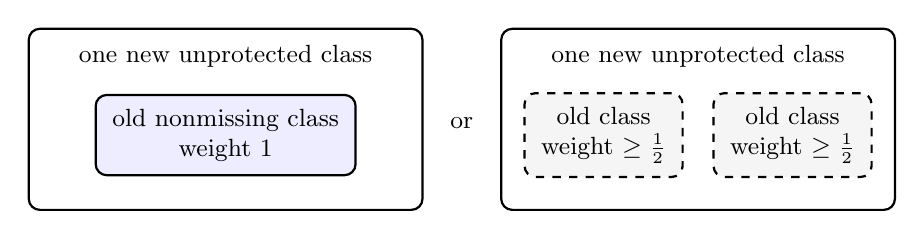
\begin{tikzpicture}[font=\small,thick]
 \draw[rounded corners] (0,0) rectangle (5,2.3);
 \draw[rounded corners] (6,0) rectangle (11,2.3);
 \node at (2.5,1.95) {one new unprotected class};
 \node at (8.5,1.95) {one new unprotected class};
 \node[draw,rounded corners,fill=blue!7,align=center,
       inner xsep=6pt,inner ysep=5pt] at (2.5,0.95)
       {old nonmissing class\\weight $1$};
 \node[draw,dashed,rounded corners,fill=black!4,align=center,
       inner xsep=6pt,inner ysep=5pt] at (7.3,0.95)
       {old class\\weight $\ge\frac12$};
 \node[draw,dashed,rounded corners,fill=black!4,align=center,
       inner xsep=6pt,inner ysep=5pt] at (9.7,0.95)
       {old class\\weight $\ge\frac12$};
 \node at (5.5,1.1) {or};
\end{tikzpicture}
\caption{The weighted containment argument in the chain bound. All
classes shown have one fixed sign and contain no protected label.
Each new class contains either a whole nonmissing old class or two
distinct whole old classes. A missing old class has weight $1/2$;
every other old class has weight $1$. The displayed regions express
set containment schematically. Distinct new classes cannot use the
same whole old class, so their unit weight requirements add.}
\label{fig:nesting-budget}
\end{figure}


By Lemma~\ref{nest:containment}, each unprotected class at stage $j$
contains previous classes of total weight at least $1$:
either one nonmissing class, or two distinct classes.
Every contained previous class is unprotected, since a protected
label in it would also protect the new class.
Distinct new classes cannot use the same previous class, because
classes of a fixed sign are disjoint and the two sign-label sets
are disjoint. Consequently
\[
 s_j\leq s_{j-1}-\frac{\delta_j}{2}.
\]
Summing and using $s_k\geq0$ yields
$\sum_{j=1}^k\delta_j\leq2(s_0-s_k)\leq2|J_0|$.
\end{proof}
